% begin module rational-functions
\begin{frame}
\frametitle{Rational Functions}
\begin{definition}[Rational Function]
A rational function is a quotient of two polynomials; that is, a function of the form
\[
f(x) = \frac{g(x)}{h(x)},
\]
where $g$ and $h$ are polynomials.
\end{definition}
\begin{columns}[c]
\column{.4\textwidth}
\uncover<2->{
\psset{xunit=0.4cm, yunit=0.4cm}
\begin{pspicture}(-5, -5)(5,5) 
\psframe*[linecolor=white](-5,-5)(5,5) 
\psaxes[ticks=none, labels=none]{<->}(0,0)(-4.5,-4.5)(4.5,4.5)\tiny
%Function formula: \frac{x}{(x)^{2}-1} 
\rput(2.5,-3){$y=\frac{x}{x^{2}-1}$} 
\psplot[linecolor=red, plotpoints=1000]{1.11727}{4.5}{x -1 x 2 exp add div } %Function formula: \frac{x}{(x)^{2}-1} 
\psplot[linecolor=red, plotpoints=1000]{-0.895043}{0.895043}{x -1 x 2 exp add div } %Function formula: \frac{x}{(x)^{2}-1} 
\psplot[linecolor=red, plotpoints=1000]{-4.5}{-1.11727}{x -1 x 2 exp add div }
\psLabels{4.5}{4.5}
\end{pspicture} 
%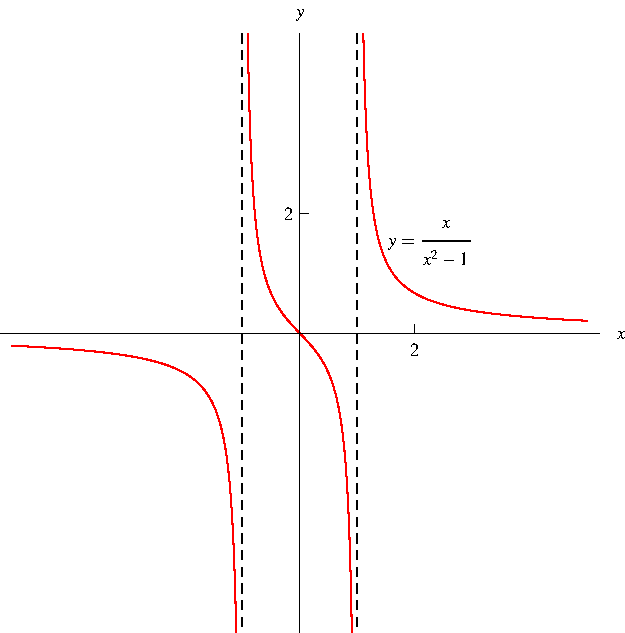
\includegraphics[height=4cm]{precalculus/pictures/01-02-rational.pdf}%
}
\column{.6\textwidth}
\uncover<2->{
\begin{example}[$x/(x^2-1)$]
The function
\[
f(x) = \frac{x}{x^2-1}
\]
is a rational function.
\end{example}
}
\end{columns}
\end{frame}
% end module rational-functions
